%
% Introduction
%
\section{Introdução}


%
% Community emvolvment
%
\begin{frame}\frametitle{Apresentação}

	\begin{figure}[h]
        \centering
        
\includegraphics[scale=0.25]{images/community.png}
    \end{figure}
\end{frame}

%
% SDN
%
\begin{frame}\frametitle{SDN}

    \begin{itemize}
    \item Software Defined Networking (Redes definidas por software)
    \end{itemize}
    	\begin{figure}[h]
        \centering
        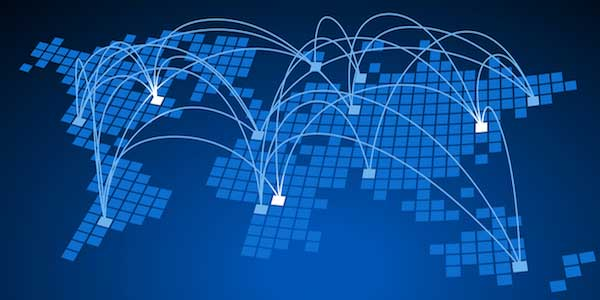
\includegraphics[scale=0.5]{images/sdn.jpg}
    \end{figure}
\end{frame}


%
% SDN
%
\begin{frame}\frametitle{SDN}

    \begin{itemize}
    \item Separa o plano de \emph{dados} do plano de \emph{controle}
    \end{itemize}
    	\begin{figure}[h]
        \centering
        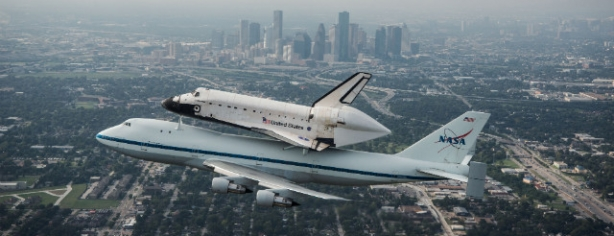
\includegraphics[scale=0.5]{images/planes.jpg}
    \end{figure}
\end{frame}


%
% Data plane
%
\begin{frame}\frametitle{Data Plane}

    \begin{itemize}
    \item Encaminhamento de pacotes
    \item Comutação no \emph{hardware} do \emph{switch}
    \end{itemize}
    	\begin{figure}[h]
        \centering
        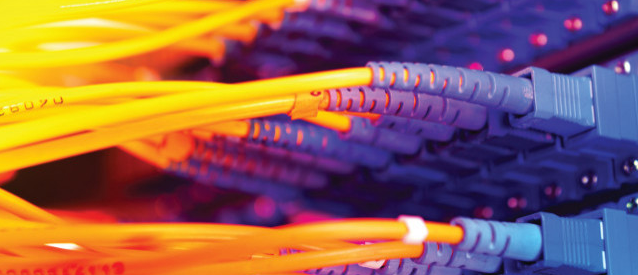
\includegraphics[scale=2.0]{images/data-plane.png}
    \end{figure}
\end{frame}


%
% Control plane
%
\begin{frame}\frametitle{Control Plane}

    \begin{itemize}
    \item Decidir como encaminhar os pacotes
    \item Roteamento, políticas e visão topológica
    \end{itemize}
    	\begin{figure}[h]
        \centering
        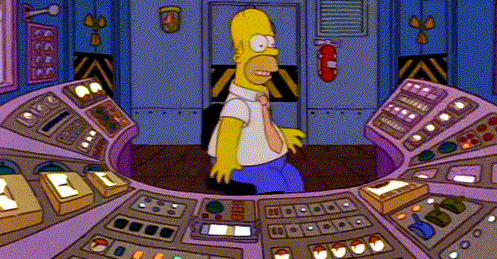
\includegraphics[scale=0.5]{images/control-plane.png}
    \end{figure}
\end{frame}


